\documentclass[11pt]{article}
\usepackage[english]{babel}
\usepackage{geometry}
\usepackage{amsmath}
\usepackage{amsthm}
\usepackage{graphicx}
\usepackage[utf8]{inputenc}

%%%%%%%% MARGIN
\geometry{verbose, letterpaper, tmargin=3cm,
  bmargin=3cm,lmargin=2.5cm,rmargin=2.5cm}

%%%%%%%% PARAGRAPH SETTINGS
% https://tex.stackexchange.com/questions/27802/set-noindent-for-entire-file
\setlength\parindent{0pt}

% https://tex.stackexchange.com/questions/49188/how-to-insert-vertical-space-between-paragraphs
\setlength{\parskip}{5pt}

%%%%%%%% SUB-FIGURE PACKAGE
\usepackage{subcaption}

%%%%%%%% HYPERREF PACKAGE
\usepackage{hyperref}
\hypersetup{linkcolor=blue}
\hypersetup{citecolor=blue}
\hypersetup{urlcolor=blue}
\hypersetup{colorlinks=true}

%%%%%%%% DEFINITION AND THEOREM DEFINITIONS
\theoremstyle{definition}
\newtheorem{definition}{Definition}[section]

\theoremstyle{remark}
\newtheorem{remark}{Remark}

\theoremstyle{remark}
\newtheorem{question}{Question}

\newtheorem{theorem}{Theorem}[section]

%%%%%%%% MULTI-COLUMNS PACKAGE
\usepackage{multicol}

%%%%%%%% BIB-LATEX STUFF
\usepackage[style=numeric,
            bibstyle=numeric,
            citestyle=numeric,
            hyperref=true,
            backend=biber]{biblatex}
\addbibresource{ref.bib} %Put relative path to ref

%%%%%%%% PERSONAL COMMANDS
\usepackage{amssymb}

%%%% Important sets
\renewcommand{\O}{\mathbb{O}}
\newcommand{\N}{\mathbb{N}}
\newcommand{\Z}{{\mathbb{Z}}}
\newcommand{\Q}{{\mathbb{Q}}}
\newcommand{\R}{{\mathbb{R}}}

%%%% Usual operations
\newcommand{\pow}[2]{#1^{#2}}
\newcommand{\expp}[1]{e^{#1}}
\newcommand{\fst}{\mathrm{fst}}
\newcommand{\snd}{\mathrm{snd}}

%%%% Lambda Calculus
\newcommand{\dneq}{\,\, \# \,\,}
\renewcommand{\S}{\pmb{\mathrm{S}}}
\newcommand{\I}{\pmb{\mathrm{I}}}
\newcommand{\K}{\pmb{\mathrm{K}}}
\newcommand{\ch}[1]{\ulcorner #1 \urcorner}

%%%% Ordinal Lambda Calculus
\newcommand{\ordAlph}{\Sigma_{\text{Ord}}}
\newcommand{\termOrd}{\text{Term}_\text{Ord}}
\newcommand{\fl}{\mathrm{fl}}
\newcommand{\sk}{\mathrm{sk}}

%% Superscript to the left
% https://latex.org/forum/viewtopic.php?t=455
\usepackage{tensor}
\newcommand{\app}[3]{\tensor*[^{#1}]{\left(#2, #3\right)}{}}

%%%% Make optional parameter
% https://tex.stackexchange.com/questions/217757/special-behavior-if-optional-argument-is-not-passed
\usepackage{xparse}

%%%% Statistics
\NewDocumentCommand{\E}{o m}{
  \IfNoValueTF{#1}
  {\mathbb{E}\left[#2\right]}
  {\mathbb{E}^{#1}\left[ #2\right]}
}
\NewDocumentCommand{\V}{o m}{
  \IfNoValueTF{#1}
  {\mathrm{Var}\left[#2\right]}
  {\mathrm{Var}^{#1}\left[ #2\right]}
}
\RenewDocumentCommand{\P}{o o m}{
  \IfNoValueTF{#1}
  {\IfNoValueTF{#2}
    {\mathrm{P}\left(#3\right)}
    {\mathrm{P}^{#2}\left(#3\right)}}
  {\IfNoValueTF{#2}
    {\mathrm{P}_{#1}\left(#3\right)}
    {\mathrm{P}_{#1}^{#2} \left(#3\right)}}
}

%%%% Lambda Calculus
\NewDocumentCommand{\cx}{o}{
  \IfNoValueTF{#1}
  {\left[\quad\right]}
  {\left[\, #1 \,\right]}
}

%%%% Create absolute value function
% https://tex.stackexchange.com/questions/43008/absolute-value-symbols
\usepackage{mathtools}
\DeclarePairedDelimiter\abs{\lvert}{\rvert}%
\DeclarePairedDelimiter\norm{\lVert}{\rVert}%
\makeatletter
\let\oldabs\abs
\def\abs{\@ifstar{\oldabs}{\oldabs*}}
%
\let\oldnorm\norm
\def\norm{\@ifstar{\oldnorm}{\oldnorm*}}
\makeatother

%%%%%%%% LOGIC TREES
\usepackage{prftree}

%%%%%%%% SPLIT EQUATIONS
% https://tex.stackexchange.com/questions/51682/is-it-possible-to-pagebreak-aligned-equations
\allowdisplaybreaks

%%%%%%%% FLOAT SPECIFIER
% https://www.overleaf.com/learn/latex/Errors/LaTeX_Error:_Unknown_float_option_%60H%27
\usepackage{float}

%%%%%%%% TO USE SHORT COMMANDS FOR VECTOR LINES
\usepackage{esvect}

%%%%%%%% ENUMERATE LABEL
% https://www.latex-tutorial.com/tutorials/lists/
\usepackage{enumitem}

%%%%%%%% DIFFERENT FONTS FOR MATH
\usepackage{mathrsfs}

%%%%%%%% CODE RENDERING !!! UNCOMMENT IF NEEDED !!!
% Compile with flag -shell-escape
%\usepackage{minted}

%%%%%%%% START DOCUMENT
\title{Stochastic Processes II: Final Report}
\author{Juan Sebasti\'an C\'ardenas-Rodríguez \\
       David Plazas Escudero \\
       \scalebox{0.7}{Mathematical Engineering, Universidad EAFIT}}
\date{June 11, 2020}

\begin{document}
\maketitle
The code for this workshop can be found in the
\href{https://github.com/Daples/JuanSePlazas/blob/master/201/stochastic-process-2/homework-2/src.py}{source
  code}.

\section*{Option Assessment}
\begin{question}
  Select a financial action that does not pay dividends, for a full operation
  year. Make a complete description if the company, specifying the type of
  operation, market, etc. Additionally, verify that the price of the selected
  action follows a lognormal distribution, based on statistical tests.
\end{question}

The selected company was Facebook. According to Facebook's company profile in
Bloomberg, ``\textit{Facebook, Inc. operates a social networking website. The
  Company website allows people to communicate with their family, friends, and
  coworkers. Facebook develops technologies that facilitate the sharing of
  information, photographs, website links, and videos. Facebook users have the
  ability to share and restrict information based on their own specific
  criteria.}'' \parencite{fb_bloom} It started as a website in Harvard
University in 2004, developed by Mark Zuckerberg \cite{guardian} and it rapidly
grew into a worldwide company. The main products of Facebook Inc. include
Facebook, Instagram, Messenger, WhatsApp and Oculus \parencite{reu}.

The prices were obtained from the
\href{https://finance.yahoo.com/quote/FB/history?p=FB}{Yahoo Finance page for
  Facebook Inc.}. The obtained time series is presented in Figure
\ref{fig:ts_prices}.

\begin{figure}[H]
    \centering
    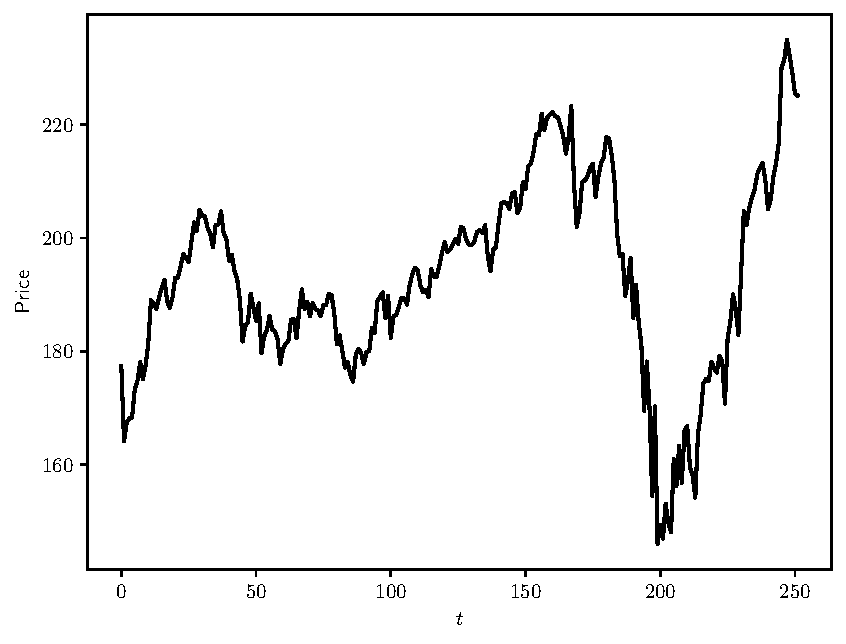
\includegraphics[scale=0.5]{../plts/prices_ts.pdf}
    \caption{Time Series of Facebook Inc. prices.}
    \label{fig:ts_prices}
\end{figure}

In order to verify that the selected action follows a lognormal distribution, a
standard Kolmogorov-Smirnov goodness-of-fit test and we obtained a p-value of
$0.764$, which implies that there is evidence to affirm that the prices follow a
lognormal distribution (and a good fit, since the pvalue is high). Furthermore,
the histogram and the fitted lognormal distribution are presented in Figure
\ref{fig:hist_log_prices}.

\begin{figure}[H]
    \centering
    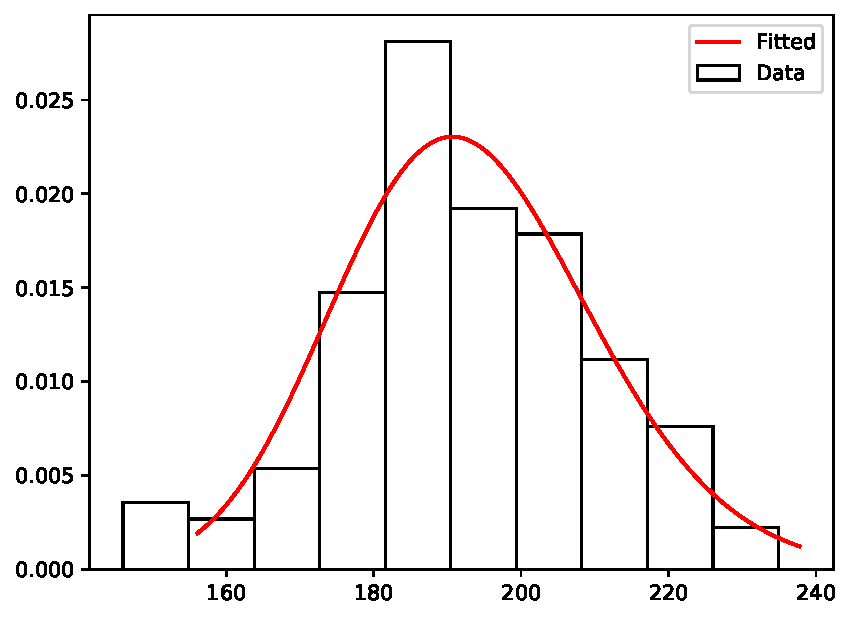
\includegraphics[scale=0.5]{../plts/price_fitting.pdf}
    \caption{Histogram and lognormal distribution of prices.}
    \label{fig:hist_log_prices}
\end{figure}

Finally, the empirical and theoretical cumulative distribution functions, as
well as the 95\% confidence bands for the empirical distribution, are presented
in Figure \ref{fig:ecdfs}. The confidence bands where calculated using the
Dvoretzky-Kiefer-Wolfowitz inequality (see e.g. \parencite{wasserman2006}). The
authors consider that the presented results give strong evidence that the prices
follow a lognormal distribution.

\begin{figure}[H]
    \centering
    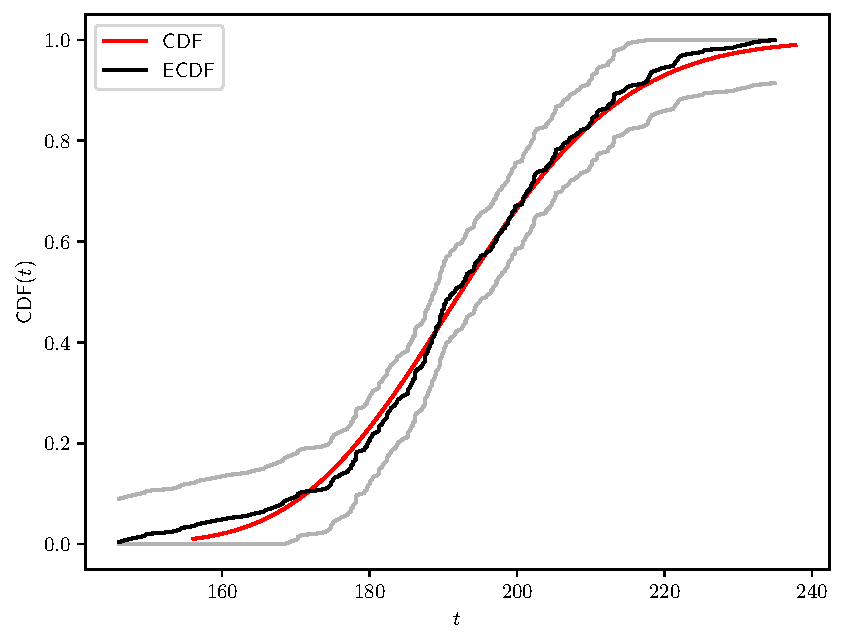
\includegraphics[scale=0.5]{../plts/ecdf.pdf}
    \caption{Cumulative distributions functions.}
    \label{fig:ecdfs}
\end{figure}

\begin{question}
  Consult the risk-free interest rate for the financial market to which the
  selected action belongs. Additionally, estimate the volatility of the action
  returns using the maximum likelihood methodology studied in class.
\end{question}

The free risk rate of Facebook was taken from \href{https://bit.ly/30yrDY4}{Guru
  Focus}. The free risk rate was extracted from the website on the 2nd of June
of 2020. The value for this rate is $r = 0.65\%$.

On the other hand, the volatility was estimated by using the Maximum Likelihood
methodology. Let $y_{i}$ for $i = 1, 2, \ldots, n$ be the prices of the stock.
Then, in the first place, the returns $\omega_{i}$ are calculated by:
\begin{equation*}
  \omega_{i} = \frac{y_{i + 1} - y_{i}}{y_{i}}
\end{equation*}
It is important to remark that the amount of returns is one less than the data.
The time series for the returns can be seen in Figure \ref{fig:rtjs}. Finally,
the volatility $\sigma$ is estimated by the following equation:
\begin{equation*}
  \sigma = \frac{1}{(n - 2) \Delta t} \sum_{i = 1}^{n - 1}\left(\omega_{i} -
    \frac{1}{n - 1}\sum_{i=1}^{n - 1} \omega_{i}\right)^{2}
\end{equation*}
The result for this estimation is $\sigma = 0.025$.

\begin{figure}[ht]
  \centering
  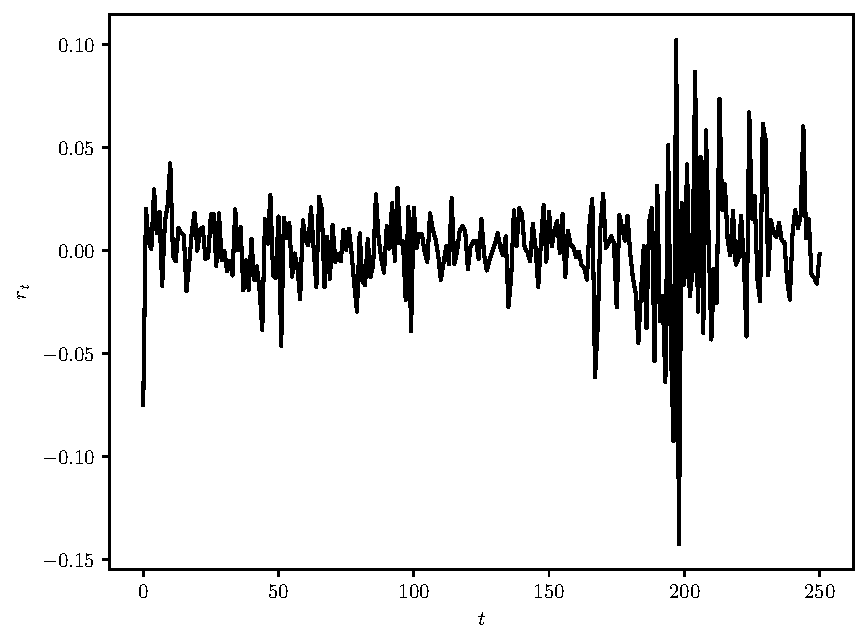
\includegraphics[scale=.5]{../plts/returns_js}
  \caption{Time series for returns used for ML methology.}
  \label{fig:rtjs}
\end{figure}
\begin{question}
  Use the Black-Scholes formula to evaluate an \textbf{European call} option,
  where the underlying is the selected action (this will be named \textit{Option
    1}). Evaluate this option for an expiry of 1 year and three different
  strikes. The strikes must be selected such that the option could be executed
  ($S_0>K$). Compare the results with the ones obtained using Montecarlo, finite
  differences and binomial trees. Analyze the results.
\end{question}

The stock pricing was realized with Black-Scholes, Monte Carlo simulation,
binomial trees, and finite differences. The pricing obtained with Black-Scholes
is considered to be the exact pricing for the Facebook stock.

\textcite{black1973} created a methodology to correctly price a European call
option. Nowadays, this methodology is known as the Black-Scholes method. Let
$\sigma$ be the volatility of the stock, $T$ the time for that option. Then, two
quantiles are calculated by:
\begin{equation*}
  d_{1} = \frac{1}{\sigma \sqrt{T}} \left(\log\left(\frac{S_{0}}{K}\right)
    + \left(r + \frac{1}{2}\sigma^{2}\right) T\right), \qquad d_{2} = d_{1} - \sigma \sqrt{T}
\end{equation*}
Lastly, using these quantiles the pricing for the option $f$ is calculated as follows:
\begin{equation*}
  f = S_{0} F(d_{1}) - K \expp{-rT} F(d_{2})
\end{equation*}

with $F(\cdot)$ the continuous distribution function for a standard normal
distribution.

The second method used was a Monte Carlo simulation approach. This approach was
created by \textcite{boyle1977}. The Monte Carlo simulation method first
simulates the selected differential equation with $M$ trajectories. In the case
of the returns, the process is a Geometric Brownian Motion, which is discretized
as:
\begin{equation*}
  S_{t + \Delta t} = S_{t}\expp{\left(r - \frac{\sigma^{2}}{2}\right) + \sigma \Delta B_{t}}
\end{equation*}
Then, the payoff is calculated by:
\begin{equation*}
  p_{i} = \max(S_{i,T} - K, 0)
\end{equation*}
Consequently, then the $f_{\text{call}}$ is calculated by the following
equation:
\begin{equation*}
  f_{\text{call}} = e^{-rT} \E{p}
\end{equation*}
This process is repeated $W$ times, saving the results of each simulation.
Finally, the mean of all the $f_{\text{call}}$ is calculated to estimate the
pricing of the option.

The Finite Differences method consists in calculating the values for a grid of a
given size. The grid has a size of $NT \times NS$, where $NS$ is the number of
$S$ to be simulated and $NT$ is the number of sample of times to be considered.

In the first place, three barrier conditions are calculated. Which are:
\begin{align*}
  f_{NT, j} &= \max(j \Delta s - K, 0) \\
  f_{j, NS} &= \max(S_{max} - K, 0) \\
  f_{j, 0} &= 0
\end{align*}
where $S_{max} = 3S_{0}$ and $\Delta s = S_{max} / NS$. Finally, the rest of the
grid is calculated based on the row forward, the equation is:
\begin{equation*}
  f_{i, j} = a_{j} f_{i+1, j-1} + b_{j} f_{i + 1, j} + c_{j} f_{i+1, j+1}
\end{equation*}
where
\begin{align*}
  a_{j} &= \frac{\Delta t}{r \Delta t + 1} \left(\frac{1}{2}\sigma^{2} j^{2}
          - \frac{1}{2}j\right) \\
  b_{j} &= \frac{\Delta t}{r \Delta t + 1} \left(\frac{1}{\Delta t} - \sigma^{2}
          j^{2}\right) \\
  c_{j} &= \frac{\Delta t}{r \Delta t + 1} \left(\frac{1}{2}\sigma^{2}j^{2} +
          \frac{1}{2}rj\right)
\end{align*}
The Binomial Tree method was created by \textcite{cox1979}. This method consists
of defining a barrier for a binomial tree and, then calculating the value for
the root by regressing. An example of a binomial tree can be seen in Figure
\ref{fig:btex}.

\begin{figure}[ht]
  \centering
  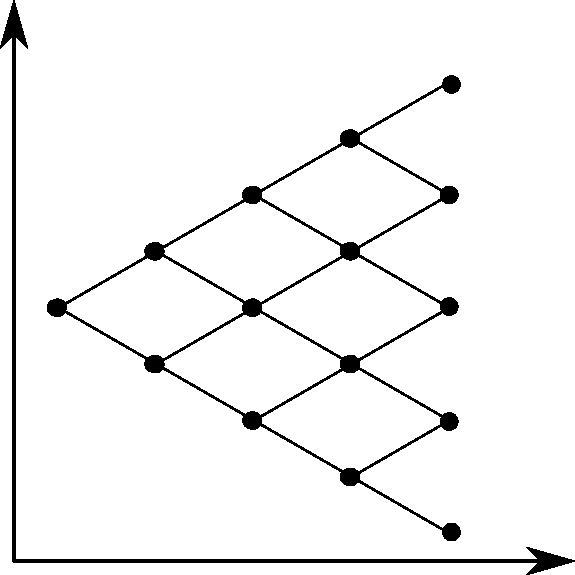
\includegraphics[scale=.5]{../plts/binomial-tree-example}
  \caption{Example of binomial tree}
  \label{fig:btex}
\end{figure}

Let $N$ be the depth of the binomial tree, i.e. the number of nodes from the
root to the last node. In the first place, the barrier is calculated by:
\begin{equation*}
  f_{N, j} = \max(S_{0}ujd(N - j) - K, 0)
\end{equation*}
with:
\begin{equation*}
  u = \expp{\sigma \sqrt{\Delta t}}, \quad d = \expp{-\sigma \sqrt{\Delta t}}, \quad
  p = \frac{\expp{r \Delta t} - d}{u - d}
\end{equation*}

Lastly, the tree is traversed backwards calculating each node by:
\begin{equation*}
  f_{i, j} = \expp{-r \Delta t} (p f_{i + 1, j+1} + (1 - p)  f_{i+1, j})
\end{equation*}

The pricing for the option is stored in the root of the tree, after completing
all calculations.

Three strikes where selected such that for each $K$ it happens that $S_0 > K$,
with $S_0 \approx 225$. The strikes with the comparison of the result of each
method is shown in Table \ref{tab:comp1}. For Monte Carlo, the selected
parameters were $M=3000$ and $W=500$. For finite differences, the selected
parameter was $NS = 1000$. Finally, for the binomial tree the selected parameter
was $N=100$.

\begin{table}[H]
\centering
\begin{tabular}{ccccc}
\hline
        & Black Scholes & Monte Carlo & Finite Diffs. & Binomial Tree \\
$K=200$ & 186.22        & 184.70      & 157.52        & 186.22        \\
$K=100$ & 205.65        & 204.29      & 191.91        & 205.65        \\
$K=50$  & 215.37        & 213.81      & 208.03        & 215.37        \\ \hline
\end{tabular}
\caption{Result for each method for two decimal places.}
\label{tab:comp1}
\end{table}

The method which was the closest one to the exact solution was the Binomial Tree
as the numbers are equal to two decimals. Then, it is followed by the Monte
Carlo simulation method, which was the second closest but the slowest algorithm.
Finally, the Finite Difference was the worst at estimating the pricing. In this
manner, by this small experiment, it can be stated that Binomial Tree is the
most precise and efficient method.

It is important to notice, that the result of each method is the pricing for the
respective derivative. Hence, it is important to see that for smaller values of
$K$ the price of the derivative becomes bigger. This happens because a smaller
strike value would increase the price of the derivative.
\begin{question}
  Suppose that you want to evaluate an \textbf{European call} option with the
  returns of the action selected (this will be named \textit{Option 2}).
  Identify and justify the selection of the stochastic differential equation
  that models these returns. Evaluate the option considering three possible
  strikes, using a parameter for the proportionality of the market's risk,
  between 10\% and 15\%. Analyze the results.
\end{question}


For each method, a time series for the returns are calculated. Differently to
the previous question, the returns are calculated by:
\begin{equation*}
  \omega_{i} = \log\left(\frac{y_{i + 1}}{y_{i}}\right)
\end{equation*}
with $y_{i}$ are the prices for the Facebook stock. Furthermore, it is important
to notice that this returns also have one less data than the stock prices. This
returns have to distribute normally. So, a fitting was made and tested by using
Kolmorogov-Smirnov test, this test failed. The histogram for the fitting and the
returns can be seen in Figure \ref{fig:rth}.

\begin{figure}[ht]
  \centering
  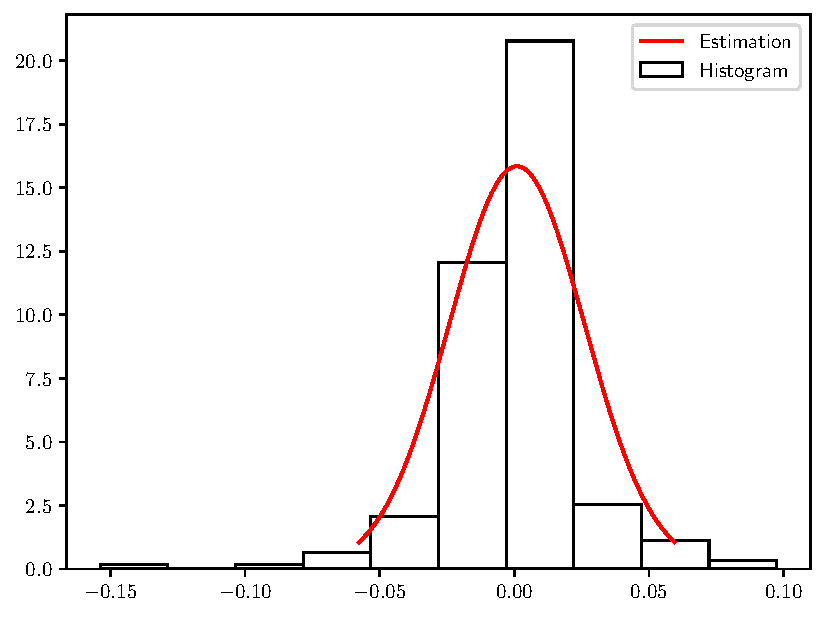
\includegraphics[scale=.5]{../plts/return_fitting}
  \caption{Histogram and fitting for returns.}
  \label{fig:rth}
\end{figure}

Although the test failed, it is seen that the fitting works quite well. The test
failed because the outliers that happen in the left tail but, for the rest of
the data the distribution is well-fitted.

Nevertheless, the stochastic process to simulate the returns was an
Ornstein-Uhlenbeck stochastic process. The parameters were estimated and the
result of the fitted process is seen in Figure \ref{fig:rtts}. The parameters
estimated were $\alpha = 1.26$, $\mu = 0.0012$, $\sigma = 0.024$ and
$\lambda=0.125$.

\begin{figure}[ht]
  \centering
  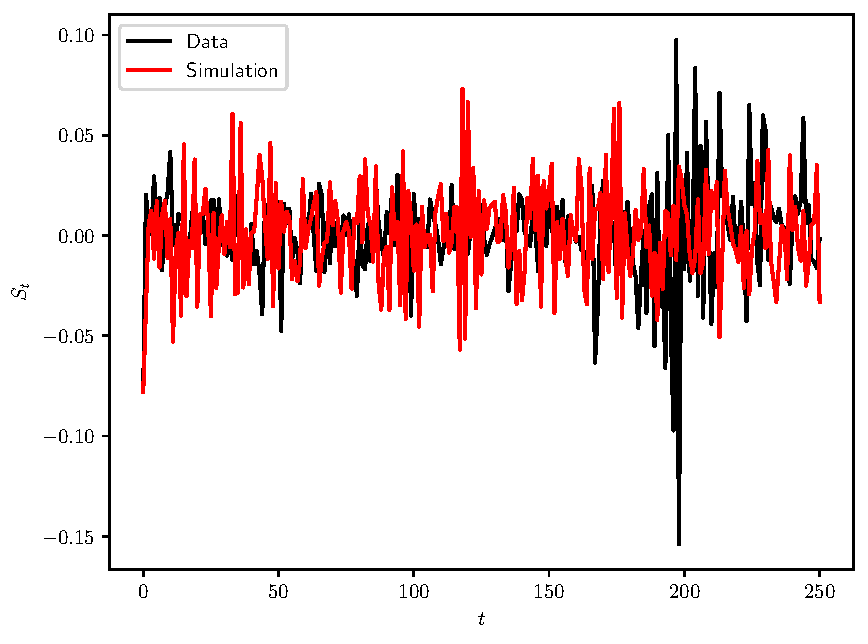
\includegraphics[scale=.5]{../plts/ou}
  \caption{Time series for returns.}
  \label{fig:rtts}
\end{figure}

To price the derivative the Monte Carlo method was used, simulating by
Euler-Maruyama's method. The result for the method can be seen in Table
\ref{tab:comp2}.

\begin{table}[H]
\centering
\begin{tabular}{cc}
\hline
         & Monte Carlo \\
$K=-0.1$ & 0.0192      \\
$K=-1$   & 0.1941      \\
$K=-3$   & 0.5829      \\ \hline
\end{tabular}
\caption{Result for each method for two decimal places.}
\label{tab:comp2}
\end{table}
\section*{Sensitivity Analysis}
Remark: all the sensitivity analysis were executed using the same parameters,
except for the one being modified. The common parameters for the sensitivity
analysis will be described: for the \textit{Option 1}, the common parameters are
$r=0.0065$, $\sigma=0.025$, $K=200$, $S_0=225.09$ and $T=252$. For the finite
differences method, $N_s=1000$ and $N_t$ is calculated by the algorithm. For the
binomial tree $N=100$. Finally, for the Montecarlo, $M=750$ and $W=125$. For the
\textit{Option 2}, $\alpha=1.258$, $\mu=0.0012$, $\sigma=0.024$,
$\lambda=0.125$, $K=-1$, $S_0=-0.00164$, $T=251$, with $M=750$ and $W=125$.
Unless stated otherwise, the parameters were modified by a $p=50\%$ factor and
taking 20 samples in the range
$[(1-p)\times\textrm{param}, (1+p)\times\textrm{param}]$.


Preserving the same financial asset defined in the last section (with their
parameters), analyze the effect on the option value of:

\begin{question}
  An increment on the expiration date ($T$). This must be verified for all
  methods for \textit{Option 1} and for Montecarlo in \textit{Option 2}.
\end{question}

This first sensitivity was done with the default parameters. In this experiment,
the objective is to find the influence that the final time of simulation $T$ has
on every method. The result for this sensitivity is found in Figure
\ref{fig:fs1}.
\begin{figure}
  \centering
  \begin{subfigure}[b]{0.45\textwidth}
    \centering
    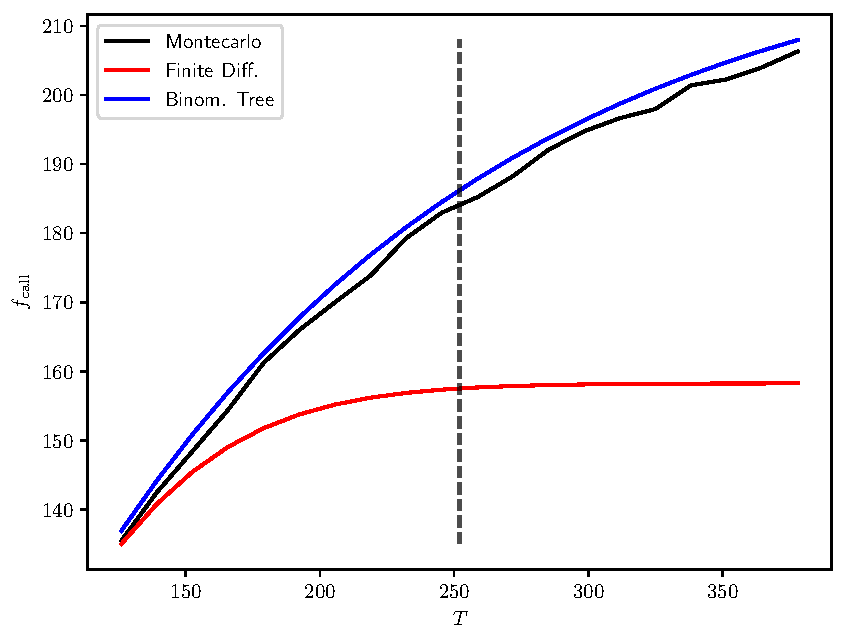
\includegraphics[scale=.5]{../plts/first_sens_opt1}
    \caption{Option 1}
  \end{subfigure}
  \begin{subfigure}[b]{0.45\textwidth}
    \centering
    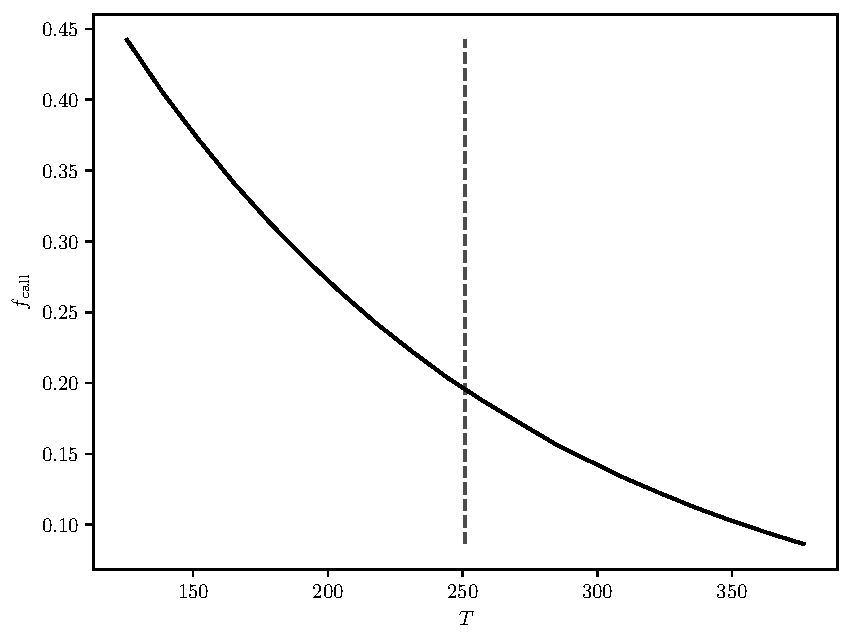
\includegraphics[scale=.5]{../plts/first_sens_opt2}
    \caption{Option 2}
  \end{subfigure}
  \caption{Results for first sensitivity for the first option.}
  \label{fig:fs1}
\end{figure}

Furthermore, it is important to see that the finite difference method does not
converge to the real solution therefore it would not be analyzed. In contrast,
the other two methods show an increase in the pricing of the derivative. This
has sense, as if the time expected to execute the derivative is larger it is
possible that the stock will have a bigger change.

On the other hand, in Figure \ref{fig:fs1} the sensitivity realized for the
second option can be seen.

The Monte Carlo simulation show a good behavior. It is seen that when the time
of simulation increases the value for the derivative decreases. This has a
similar behavior as the one shown in the previous section.
\begin{question}
  An increment on the risk-free interest rate ($r$). This must be verified for
  all methods for \textit{Option 1}.
\end{question}

This sensitivity was executed also with the default parameters. This experiment
had the objective to test the influence that the free risk rate has in the
pricing of the derivative. In Figure \ref{fig:ss}, the result for each method
can be seen.

\begin{figure}[]
  \centering
  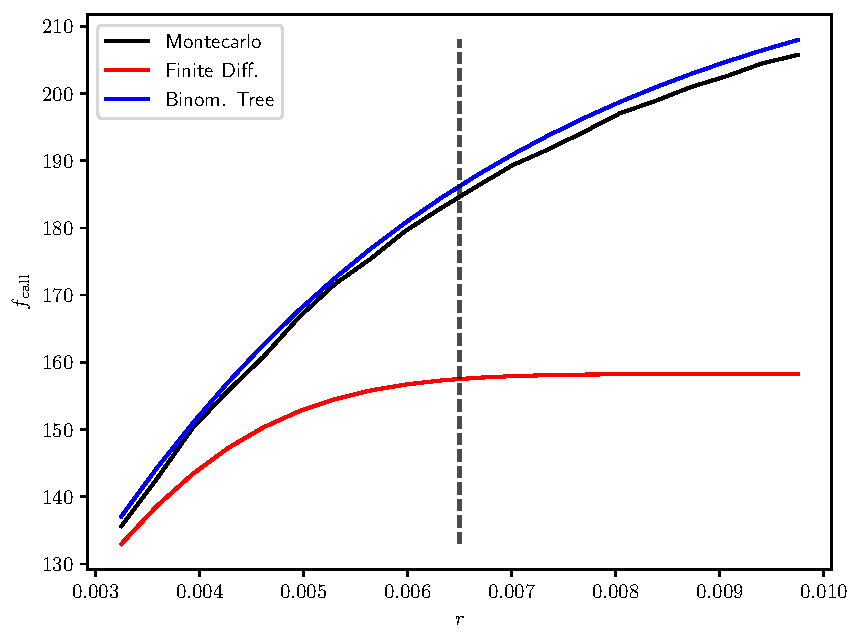
\includegraphics[scale=.5]{../plts/second_sens_opt1}
  \caption{Results for second sensitivity for first option.}
  \label{fig:ss}
\end{figure}

Similarly to the previous sensitivity, it is seen that for an increase on the
risk free rate it increases the price of the derivative. That can be easily
explained as, for a bigger rate the value of the stock should increase too. In
this manner, bigger risk free rate generates an increase in the cost of the derivative.
\begin{question}
  An increment on the volatility ($\sigma$). This must be verified for all
  methods for \textit{Option 1} and for Montecarlo in \textit{Option 2}.
\end{question}

The results for this sensitivity analysis are presented in Figure
\ref{fig:third_sens}. Recall that the volatility is a parameter directly linked
with the diffusion part in the stochastic differential equation (SDE), hence, as
sigma increases, the trajectories of the SDE will be more spread for each point
in time, i.e. the variance will increase. This can be evidenced in the lines for
the Montecarlo methods, in both Options, since they present spikes and
fluctuating behavior. Furthermore, the binomial tree method did not present any
variation on the option price for changes in the volatility. Finally, the finite
differences method showed little change in the option value, with a slight
decrease as $\sigma$ grew. For the \textit{Option 2}, the price decreases as
well, this is due to the presence of $-\lambda\sigma$ in the trend of the SDE
that models the underlying for \textit{Option 2}: as $\sigma$ increases, the
trend term tends to get smaller, and therefore, the expected return too.

\begin{figure}[H]
  \centering
  \begin{subfigure}[b]{0.45\textwidth}
      \centering
      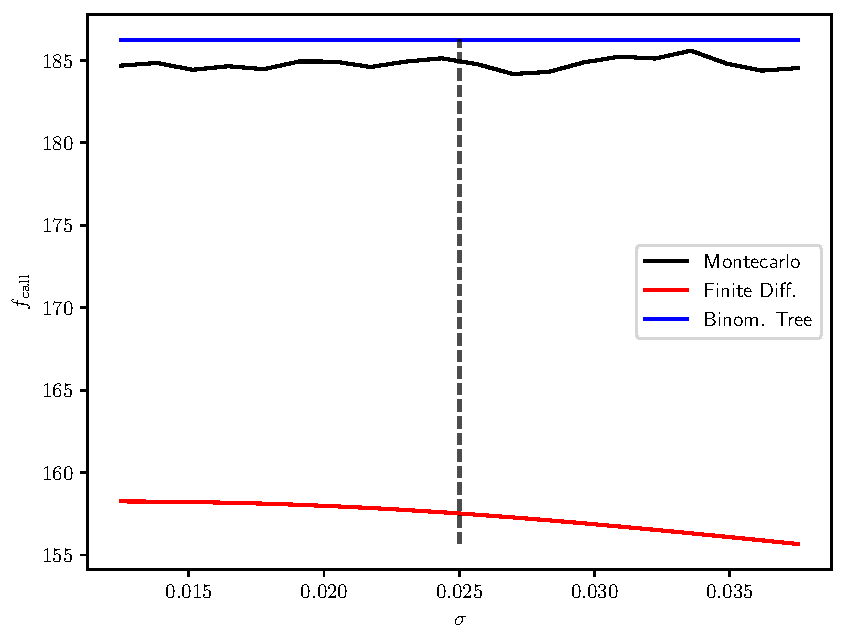
\includegraphics[scale=0.52]{../plts/third_sens_opt1.pdf}
      \caption{\textit{Option 1}.}
  \end{subfigure}
  \begin{subfigure}[b]{0.45\textwidth}
      \centering
      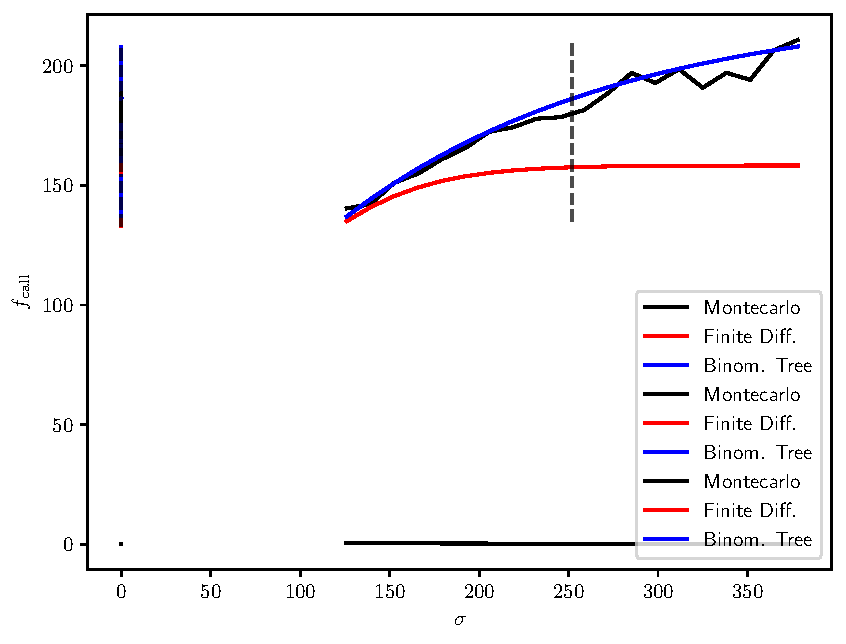
\includegraphics[scale=0.52]{../plts/third_sens_opt2.pdf}
      \caption{\textit{Option 2}.}
  \end{subfigure}
  \caption{Sensitivity on $\sigma$.}
  \label{fig:third_sens}
\end{figure}

\begin{question}
  An increment on the strike ($K$). This must be verified for all methods for
  \textit{Option 1} and for Montecarlo in \textit{Option 2}.
\end{question}

The results are presented in Figure \ref{fig:fourth_sens}. Note that for all
methods, the same results (in terms of sensitivity output) were obtained: the
option price decreases significantly as the strike $K$ increases. Taking into
consideration that these values represent the price of the contract today, as
the strike increases, it makes sense that this price decreases since the buyer
would be willing to pay more the underlying at the expiration date $T$.

\begin{figure}
  \centering
  \begin{subfigure}[b]{0.45\textwidth}
      \centering
      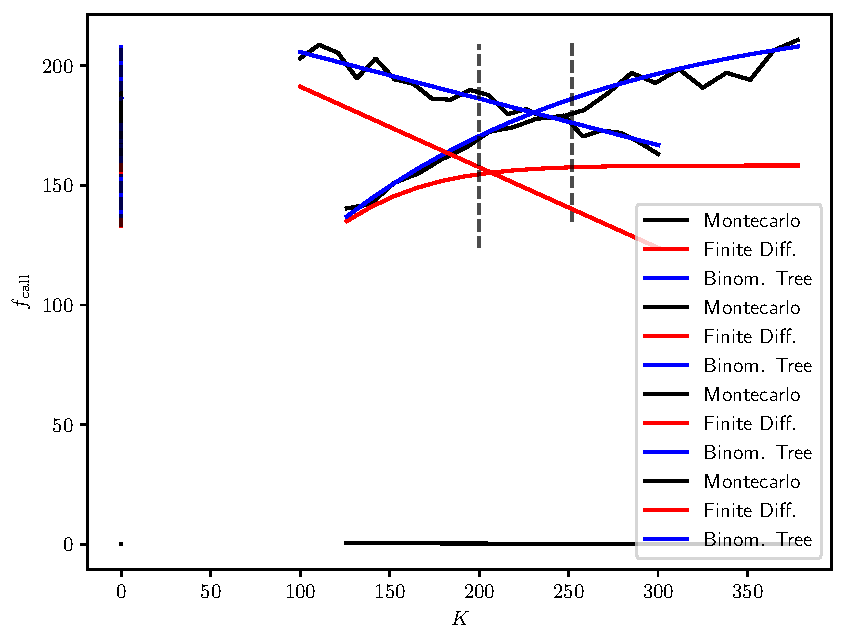
\includegraphics[scale=0.52]{../plts/fourth_sens_opt1.pdf}
      \caption{\textit{Option 1}.}
  \end{subfigure}
  \begin{subfigure}[b]{0.45\textwidth}
      \centering
      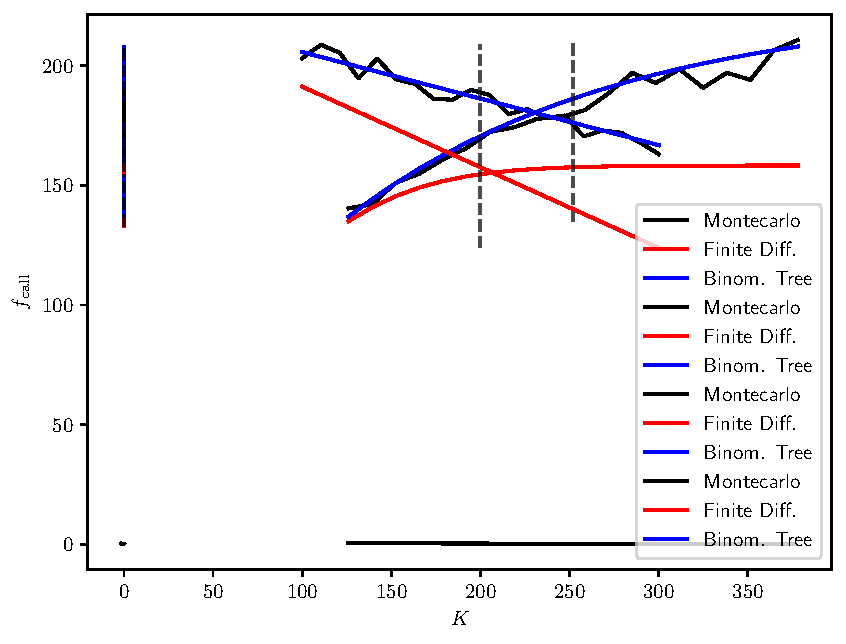
\includegraphics[scale=0.52]{../plts/fourth_sens_opt2.pdf}
      \caption{\textit{Option 2}.}
  \end{subfigure}
  \caption{Sensitivity on the strike $K$.}
  \label{fig:fourth_sens}
\end{figure}

\begin{question}
  An increment on the number of trajectories ($M$), starting in 10. An increment
  on the number of repetitions ($W$), starting in 100. An increment on the
  number of subintervals of time ($N$), starting in 100. This must be verified
  for the Montecarlo method in both \textit{Option 1} and \textit{Option 2}.
\end{question}

In Figure \ref{fig:fs51}, the result for the first experiment is seen. In this
case, it is important to remark than an increase in the parameter $M$ starts to
change the Monte Carlo simulation to oscillate around a solution. This happens
because when the number of trajectories increase, the method starts slowly
converging to the real solution. In this manner, this experiment had the
expected behavior. Furthermore, although not big enough $M$ were tested due to
computation time. it is seen that this parameter drastically improves the
convergence of the algorithm.

\begin{figure}[]
  \centering
  \begin{subfigure}[b]{0.45\textwidth}
    \centering
    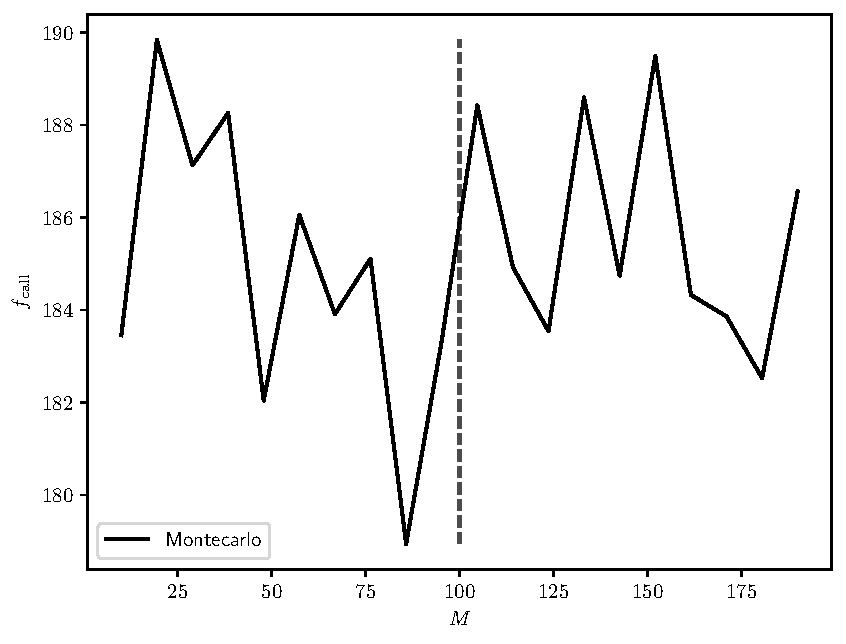
\includegraphics[scale=.5]{../plts/fifth_a_sens_opt1}
    \caption{Option 1}
  \end{subfigure}
  \begin{subfigure}[b]{0.45\textwidth}
    \centering
    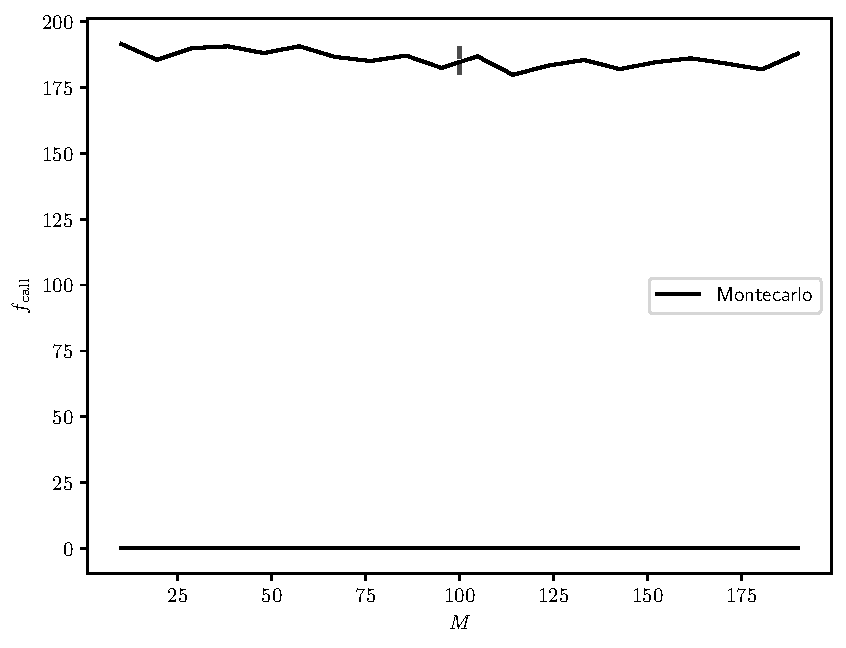
\includegraphics[scale=.5]{../plts/fifth_a_sens_opt2}
    \caption{Option 2}
  \end{subfigure}
  \caption{Results for first experiment.}
  \label{fig:fs51}
\end{figure}

In Figure \ref{fig:fs52}, the results for the second experiment are seen. For
increasing $W$, it is seen that the method tends to oscillate more around the
same point instead of stabilizing to another point. Hence, with both
experiments, one can conclude that the parameter $M$ is the one who improves the
accuracy of the method while $W$ improves the speed of convergence.

\begin{figure}[]
  \centering
  \begin{subfigure}[b]{0.45\textwidth}
    \centering
    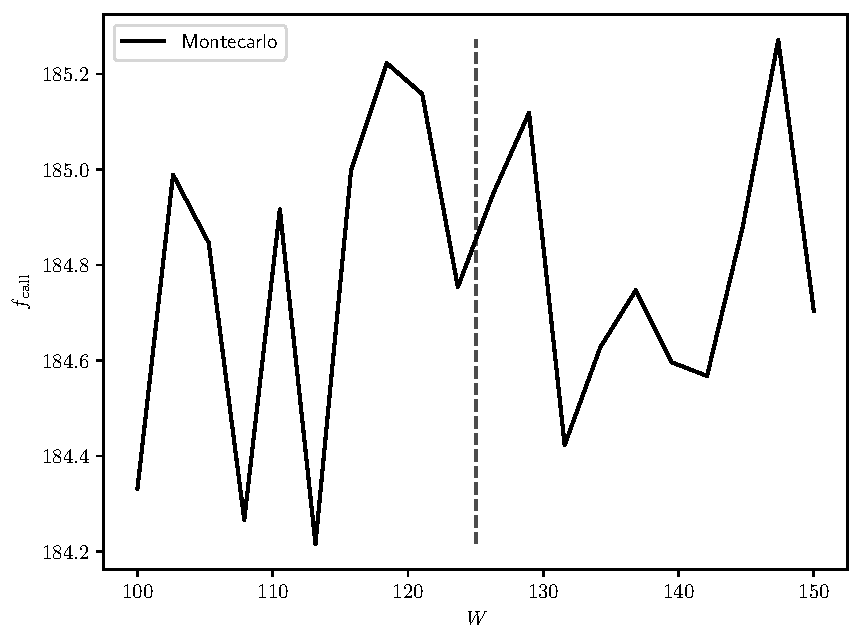
\includegraphics[scale=.5]{../plts/fifth_b_sens_opt1}
    \caption{Option 1}
  \end{subfigure}
  \begin{subfigure}[b]{0.45\textwidth}
    \centering
    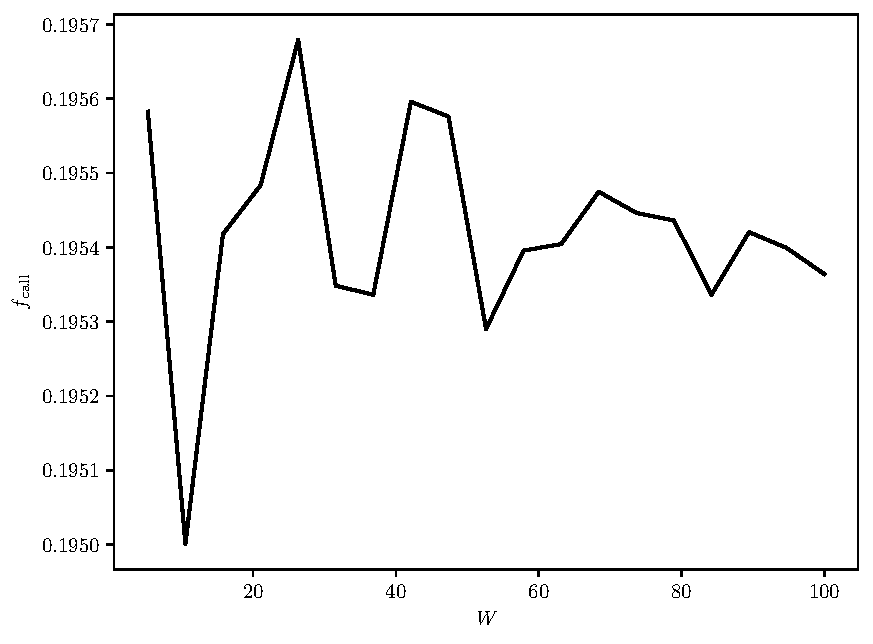
\includegraphics[scale=.5]{../plts/fifth_b_sens_opt2}
    \caption{Option 2}
  \end{subfigure}
  \caption{Results for second experiment.}
  \label{fig:fs52}
\end{figure}

Finally, in Figure \ref{fig:fs53} the results for the last experiment is seen.
It is important to remark that for both options a change in $\Delta t$ has
different impacts. In the \textit{Option 1} it is seen that an increase on
$\Delta t$ does impact the convergence of the method but it does not affect the
stability of it. On the other hand, the \textit{Option 2} does diverge as bigger
$\Delta t$ just are significantly bigger for the Euler-Maruyama method.

\begin{figure}[]
  \centering
  \begin{subfigure}[b]{0.45\textwidth}
    \centering
    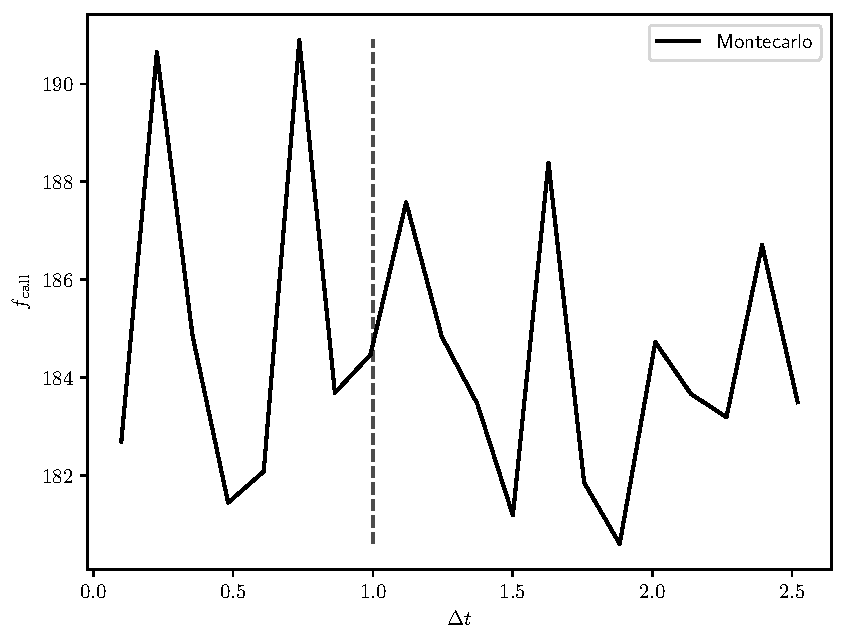
\includegraphics[scale=.5]{../plts/fifth_c_sens_opt1}
    \caption{Option 1}
  \end{subfigure}
  \begin{subfigure}[b]{0.45\textwidth}
    \centering
    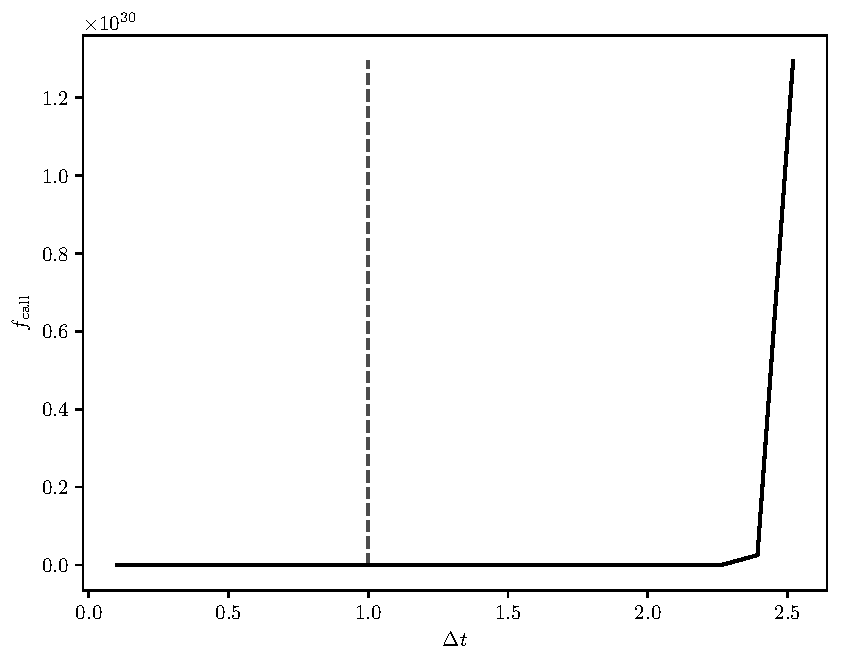
\includegraphics[scale=.5]{../plts/fifth_c_sens_opt2}
    \caption{Option 2}
  \end{subfigure}
  \caption{Results for second experiment.}
  \label{fig:fs53}
\end{figure}

\begin{question}
  An increment on the number of subintervals with respect to the underlying
  ($N_s$). This must be verified for the finite differences method for
  \textit{Option 1}.
\end{question}

Note that scale of Figure \ref{fig:sixth_sens} is relatively small, hence the
price remains on similar values. It is clear that the price appears to be
stabilizing between 157.4 and 157.6 since the amplitude of the fluctuations
appear to be getting smaller; though this is pure speculation, since it would be
needed to make more evaluations for more values for $N_s$ and a bit more
frequent to give a stronger conclusion.

\begin{figure}[H]
    \centering
    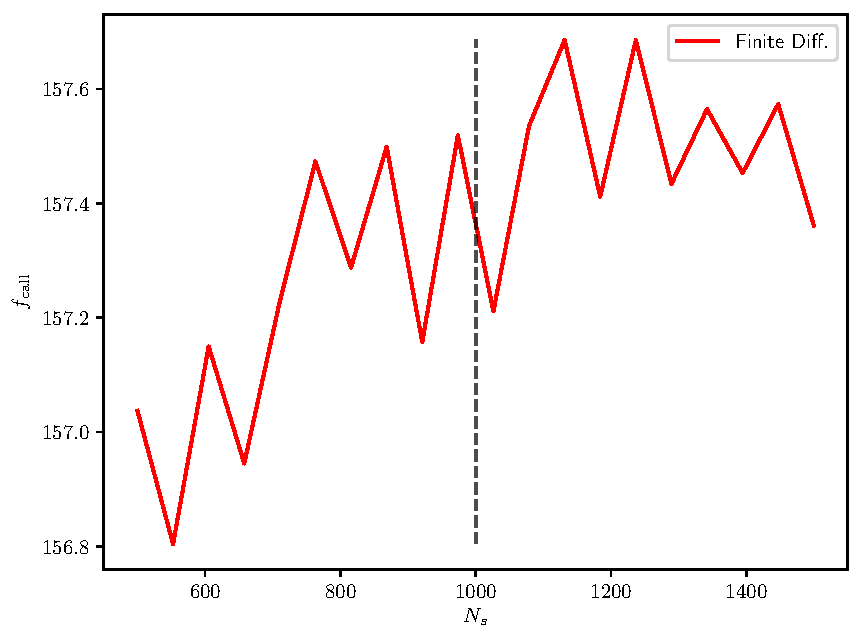
\includegraphics[scale=0.5]{../plts/sixth_sens_opt1.pdf}
    \caption{Sensitivity on $N_s$ for \textit{Option 1}.}
    \label{fig:sixth_sens}
\end{figure}

\begin{question}
  An increment in the number of subintervals in the tree with respect to time
  ($N$). this must be verified for the binomial tree method for \textit{Option
    1}.
\end{question}
Figure \ref{fig:seventh_sens} shows the results for changing the number of
subintervals in the binomial tree method for \textit{Option 1}. It can be
directly concluded that the change on the option price is insignificant (given
the scale of the vertical axis).

\begin{figure}[H]
    \centering
    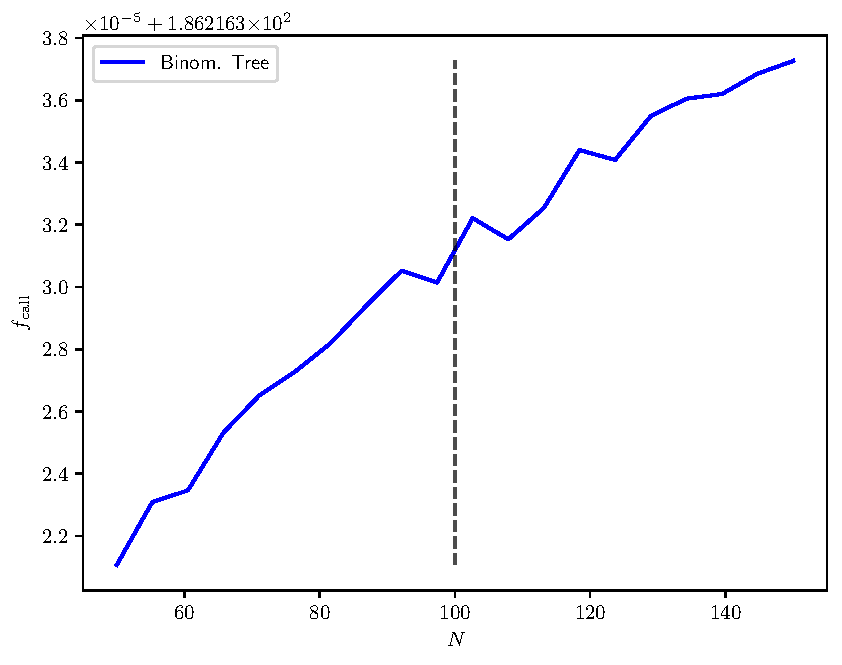
\includegraphics[scale=0.5]{../plts/seventh_sens_opt1.pdf}
    \caption{Sensitivity on $N$ for the binomial tree of \textit{Option 1}.}
    \label{fig:seventh_sens}
\end{figure}

\begin{question}
  An increment on the proportionality of the market's risk ($\lambda$). This
  must be verified for the Montecarlo method in \textit{Option 2}.
\end{question}
The results for the sensitivity on the parameter $\lambda$ can be found in
Figure \ref{fig:eight_sens}. It can be observed that the option price decreases
as $\lambda$ increases. The authors believe the this is due to the same reason
as $\sigma$: this parameter is negatively linked to the trend of the SDE,
therefore, the expected value decrements.

\begin{figure}[H]
    \centering
    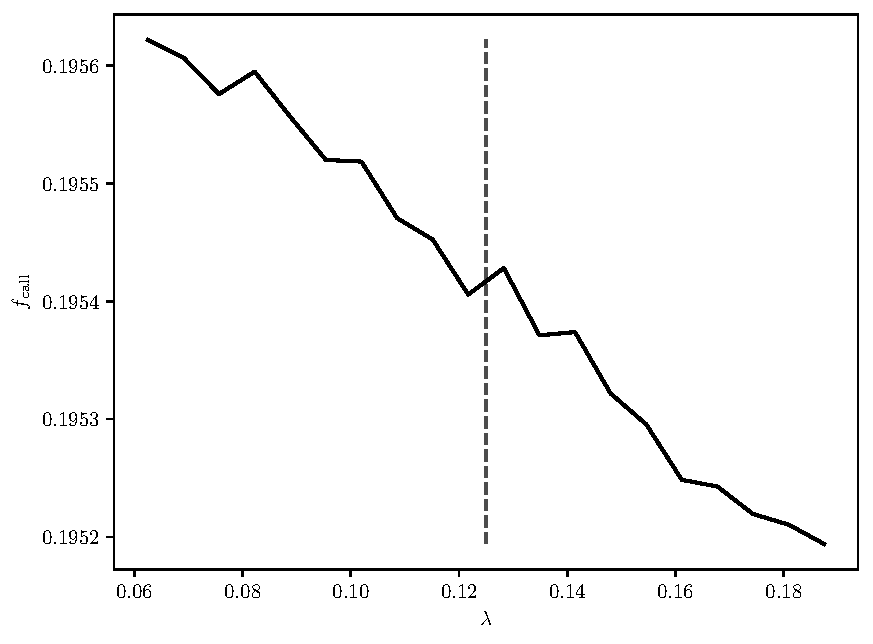
\includegraphics[scale=0.5]{../plts/eight_sens_opt2.pdf}
    \caption{Sensitivity on $\lambda$ for \textit{Option 2}.}
    \label{fig:eight_sens}
\end{figure}


\printbibliography
\end{document}
